\documentclass[conference]{IEEEtran}
\IEEEoverridecommandlockouts
% The preceding line is only needed to identify funding in the first footnote. If that is unneeded, please comment it out.
\usepackage{cite}
\usepackage{amsmath,amssymb,amsfonts}
\usepackage{algorithmic}
\usepackage{graphicx}
\usepackage{textcomp}
\usepackage{xcolor}
\usepackage{graphicx}
\usepackage{amssymb}
\graphicspath{ {figures/} }
\newcommand\numberthis{\addtocounter{equation}{1}\tag{\theequation}}
\def\BibTeX{{\rm B\kern-.05em{\sc i\kern-.025em b}\kern-.08em
    T\kern-.1667em\lower.7ex\hbox{E}\kern-.125emX}}
\begin{document}

\title{Spirogravitator\\
{\footnotesize \textsuperscript{}(University of Utah ECE 2240 Lab 2)}
}

\author{\IEEEauthorblockN{1\textsuperscript{st} Richard Baird}
\IEEEauthorblockA{\textit{IEEE Member, Student (University of Utah)} \\
\textit{University of Utah}\\
Salt Lake City, USA \\
u0977428@utah.edu}
}

\maketitle

\begin{abstract}
A fictional scenario is presented as the impetuous for solving differential equations using
Laplace transformations. The goal is explained in some detail, the circuit is analyzed, and theoretical
solutions are graphed. The circuit is built from the theoretical solutions, and the circuit is measured
and graphed.
\end{abstract}

\begin{IEEEkeywords}
laplace, circuit, analysis
\end{IEEEkeywords}

\section{Introduction}
Captain Quirk of the Starship Surprise has informed the crew that they are surrounded by Klingulon ships.
This is a perfect opportunity to test out the starship's newest weapon, the spirogravitator, heretofore referred to as "the weapon".
The weapon may only be used in a spiral, and the ship's main engineer is unable to plot the path
of the weapon owing to plot devices required to provide the opportunity for the author to plot the path instead. The path of the weapon must be plotted before it can be used. Herewith is presented the mathematical representation and solution to the weapon.

\section{Circuit Analysis}\label{sec:2}

\subsection{Deriving the symbolic equations}
Fig. 1 depicts the schematic of the weapon and introduces the two node voltages that are graphed on separate axes to create the requisite spiral pattern. the value for \textbf{L} is provided as 100$\mu$H. It is also given that $\text{C}_1 = \text{C}_2$. $V_{\textbf{i}}$ is given to be a square wave with a zero DC offset, and a frequency such that the circuit is guaranteed reach its steady-state solution before the second half of the cycle. A frequency of 100Hz is chosen for the purposes of solving the circuit.
\begin{figure}[h]
    \centering
    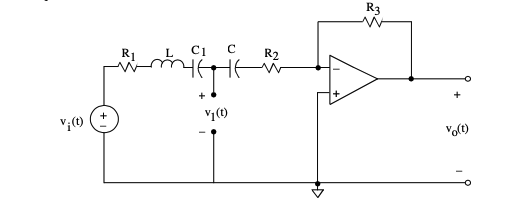
\includegraphics[scale=.45]{fig1.png}
    \caption{Diagram of the Spirogravitator circuit. $v_{\textbf{i}}$ is a rectangular wave with zero DC level.}
    \label{fig:circuit}
\end{figure}

The beginning of any circuit analysis is an appropriate Kirchoff's Voltage Law (KVL) equation. KVL provides
that the sum of all the potential differences in a closed loop are equal to zero. Thus the KVL equation for the circuit in \ref{fig:circuit} becomes
\begin{multline} \label{eq:KVL}
\sum{v_{loop}} = -v_{\textbf{i}} + iR_1 + L\frac{di}{dt} + v_{c_1}(0^+) + \frac{1}{c_1}\int_0^xi\hspace{1mm}dt\\ + {v_c}(0^+) + \frac{1}{C}\int_0^xi\hspace{1mm}dt+iR_2 = 0
\end{multline}
This equation cannot be solved with traditional linear methods without transforming the equation to a linear form. To accomplish this, a Laplace transform is used. It is trivial to show that because there are 2 capacitors of equal capacitance in series with one another, the initial voltage over each will be 1/2 the input voltage. $v_{c,c1}(0^+)$ Analyzing just the positive half of the circuit, it can be concluded that $v_{c,c1}(0^+) = -\frac{1}{2}$. The post transformation equation is shown in (2).
\begin{equation} \label{eq:LPKVL}
    \mathbb{V}_i(S) + \mathbb{I}R_1 + \mathbb{I}LS - \frac{1}{2S} +\frac{\mathbb{I}}{SC_1} - \frac{1}{2s} + \frac{\mathbb{I} }{SC} + \mathbb{I}R_2 = 0
\end{equation}
Now in a linear form, Equation \ref{eq:LPKVL} can be further simplified letting $R = R_1 + R_2$ and recalling from the given paramaters at the beginning of section \ref{sec:2} that $C_1 = C$. With these simplifications, The equation is solved for $\mathbb{I}$ in (3).
\begin{equation} \label{eq:IPartial}
\jot 4mm
\begin{split}
\mathbb{I} = \frac{S^2C^2({\mathbb{V}}_i + \frac{1}{S})}{SC^2L(S^2+\frac{RS}{L} + \frac{2}{CL})}\\ 
= \frac{S({\mathbb{V}}_i(S) + \frac{1}{S})}{L(S^2 + \frac{RS}{L} + \frac{2}{CL})}\\
= \frac{S{\mathbb{V}}_i + 1}{L(S^2 + \frac{RS}{L} + \frac{2}{CL})}
\end{split}
\end{equation}
At this point $\mathbb{I}$ can be simplified further by considering only the positive half of the cycle. That is, the portion of the cycle from time $t = 0$ to time $t = \frac{T}{2}$ where $T$ is the period of the input square wave. Taking this to be true, $v_{\textbf{i}}$ in the time domain is equal to 1V. In the Laplace domain, this translates to $1/S$. $\mathbb{I}$ can therefore be written as
\begin{equation} \label{eq:I}
\jot 4mm
    \begin{split}
    \mathbb{I} = \frac{\frac{S}{S} + \frac{S}{S}}{L(S^2 + \frac{RS}{L} + \frac{2}{CL})}\\
    = \frac{2}{L(S^2 + \frac{RS}{L} + \frac{2}{CL})}
    \end{split}
\end{equation}

With $\mathbb{I}$ solved for, ${{\mathbb{V}}_{1,2}}$ can be solved as well. For ${{\mathbb{V}}_1}$ A second KVL equation is derived by analyzing the center loop of the circuit in fig. \ref{fig:circuit} going through $v_1(t)$. Written in the Laplace domain, substituting $\mathbb{I}$ for the value found in (\ref{eq:I}), the equation is derived to be
\begin{equation} \label{eq:V1Partial}
    {\mathbb{V}}_1 = \frac{1}{2S} - \frac{2R_s}{L(S^2 + \frac{RS}{L} + \frac{2}{CL})} - \frac{2SC_0}{SL(S^2 + \frac{RS}{L} + \frac{2}{CL})}
\end{equation}

$v_o$ is much simpler. Utilizing Ohm's law, it is trivial to show that ${v_o} = -i(t)R_3$. In the Laplace domain this becomes
\begin{equation} \label{eq:VoPartial}
{\mathbb{V}}_o = -\frac{2R_3}{L(S^2 + \frac{RS}{L} + \frac{2}{CL})}
\end{equation}
\subsection{Solving the Equations}
All of the necessary equations to plot the spiral have been derived, but before they can be transformed
back to the time domain, they must be put in a form such that there exists a Laplace identity to transform
$t\implies{S}$ and vice versa. The two Identities that are the most useful are
\begin{align} \label{eq:Lcostrans}
    Ae^{-at}cos(\omega{t}) \implies A\frac{S+a}{(S+a)^2 + \omega^2}\\
    \label{eq:Lsintrans}
    Be^{-at}sin(\omega{t}) \implies B\frac{\omega}{(s+a)^2 + \omega^2}
\end{align}
Beginning with ${\mathbb{V}}_1$\textit{(\ref{eq:V1Partial})} Several manipulations must be made to get the equation in a proper form. We begin by completing the square to factor the denominator.
\begin{multline*}
    {\mathbb{V}}_1 = \frac{1}{2S} - \frac{2R_2}{L((S + \frac{R}{2L})^2 + \frac{2}{CL}- (\frac{R}{2L})^2)}\\
    - \frac{2CS}{SL((S + \frac{R}{2L})^2 + \frac{2}{CL} - (\frac{R}{2L})^2)}\\
    {}
\end{multline*}
In this form, the denominator can be represented in appropriate form from (\ref{eq:Lcostrans}) and (\ref{eq:Lsintrans}) by letting $a = \frac{R}{2L}$ and $w^2 = \frac{2}{CL}- (\frac{R}{2L})^2$.
The equation then becomes
\begin{multline} \label{eq:SandOmega}
    {\mathbb{V}}_1 = \frac{1}{2S} - \frac{2R_2}{L((S+a)^2 + w^2)} - \frac{2CS}{SL((S+a)^2 + w^2)}\\
    - A\frac{S+a}{(S+a)^2 + \omega^2}
\end{multline}
If We let $B = \frac{2R_2}{L}$ and $A = \frac{2C}{SL}$ the expression can be rewritten as 
\begin{equation*}
    {\mathbb{V}}_1 = \frac{1}{2S} - B\frac{1}{(s+a)^2 + \omega^2} - A\frac{S}{(S+a)^2 + \omega^2}
\end{equation*}
To get the equation in its final form, the second term is multiplied by $\omega/\omega$ and a term of $\frac{(a - a)}{(S+a)^2 + \omega^2}$ is added to the 3rd term. The 3rd term is then separated into 2 fractions, to arrive at the final form of equation \ref{eq:V1Partial}.
\begin{multline}\label{eq:V1Final}
    {\mathbb{V}}_1 = \frac{1}{2S} - A\frac{S+a}{(S+a)^2 + \omega^2} - B\frac{\omega}{(s+a)^2 + \omega^2}\\
    - \frac{Ba}{(S+a)^2 + w^2}
\end{multline}
The equation for ${\mathbb{V}}_o$ is much simpler to arrive at. Employing the same $\omega/\omega$ trick as seen in the previous equation, (\ref{eq:V1Final}) the final solution for $\mathbb{V}_o$ becomes
\begin{align} \label{eq:v_0 final}
    - \frac{2R_3}{L(S+\frac{R}{2L})^2 + \frac{2}{CL}-(\frac{R}{2L})^2} * \frac{\omega}{\omega}
\end{align}
Letting $A = \frac{-2R_3}{L\omega}$ and subbing the values for $\omega$ and $a$ from equation \ref{eq:SandOmega}, this equation is written in the form of identity \ref{eq:Lsintrans}.
Now with both $\mathbb{V}_0 \text{ and } \mathbb{V}_1$ in identity forms, they can be transformed back to the time domain, yielding equations
\begin{align*}
    v_o(t) = Ae^{-at}\sin{\omega{t}}\label{eq:v0t}\numberthis \\ 
    v_1(t) = \frac{1}{2} - Be^{-at}\left(\cos(\omega{t}) -\right \\
    \left\sin(\omega{t})\left(a-\frac{2R_2}{BL}\right)\right)\label{eq:v1t} \numberthis
\end{align*}
\subsection{Fitting the spiral}
It is given that in order to create the spiral, $v_1(t)$ must be of the form
\begin{equation}
    be^{-\alpha{t}}\cos(\beta{t}) + de^{-\alpha{t}} + \sin(\beta{t} + \phi) + c
\end{equation}
This is done by selecting the appropriate values for $c$, $b$, $d$, $\beta$, $\alpha$, and $\phi$. The values that will fit equation \ref{eq:v1t} are $c = \frac{1}{2}$, $b = \frac{1}{2L}$, $d = -B\left(a - \frac{2R_2}{BL}\right)$, $\beta = \omega$, $\alpha = a$, and $\phi = 0$
It is further given that in order to plot the spiral correctly, the following conditions must also be met.
\begin{align*}
    d = 0\\ \numberthis \label{eq:conditions}
    A = -B\\
    \alpha = \frac{\omega}{6\pi} = 5\text{KHz}
\end{align*}
The simplest place to begin solving for the given condition \eqref{eq:conditions} is with $\alpha$. Because $\omega$ is a radical expression, the best way to solve alpha is by squaring it first.
\begin{align*}
    \alpha^2 = \frac{\omega^2}{\left(6\pi\right)^2} = 25\text{M(Hz)}^2 \numberthis \label{eq:alpha} \\
    \implies \omega^2 = 25\text{M}*6\pi^2 \text{r/s}^2 \\
    \implies \omega = 30\text{K}\pi\text{ r/s}
\end{align*}
With $\omega$ solved, it becomes possible to solve for the capacitance C.
\begin{align*} \numberthis \label{eq:C}
    \alpha^2 = \frac{1}{CL} = \frac{\left(30\text{K}\pi\right)^2 }{2}\\
    \implies C = \frac{2}{L(30\text{K}\pi)^2} = 2.25\text{nF}\\
    C_1 = C_2 \implies C_1 + C_2 = 2C = 4.5\text{nF}
\end{align*}
The condition for $\alpha$ is also used to setup an equation for $R_1$ and $R_2$, building from \eqref{eq:SandOmega}.
\begin{align*} \numberthis \label{eq:R1+R2}
    \alpha = a = \frac{R}{2L} = \frac{R_1 + R_2}{2L} = 5{KHz}\\
    \implies R_1 + R_2 = 10L\text{K}\Omega = 1\text{K}\Omega
\end{align*}
Given the condition $d=0$ \eqref{eq:conditions} the exact values for $R_1$ and $R_2$ can be solved.
\begin{align*} \numberthis \label{eq:R1,R2}
    d = -B\omega(\frac{2R_2}{L}-\frac{2R_2}{BL} = 0 \\ 
    \implies a = \frac{2R_2}{L} \equiv \frac{R_1 + R_2}{2L} = \frac{2R_2}{L} \\
    \equiv (R_1 + R_2)  = 4R_2 = 1\text{K} \\
    \equiv R_1 = 3R_2 = 1\text{K} \\ 
    \implies R_1 = 750\Omega \text{ and } R_2 = 250\Omega
\end{align*}
From the condition \eqref{eq:conditions} $A = -B$, a value for $R_3$ is derived.
\begin{align*}
    a = -B \equiv \frac{2R_3}{2L\omega} = \frac{1}{2L} \\
    \implies R_3 = \omega/2 = 15\text{K}\pi
\end{align*}
\section{Building the circuit}
With the math complete the circuit is built using the closest to standard values available. $R_1$, $R_2$, and $R_3$ are built with series combinations of resistors to achieve the appropriate values within a $.1\%$ tolerance. Capacitors $C_1$ and $C_2$ are both designed in the same way, using a $.1\mu$F capacitor in series with a $4.7$nF capacitor, yielding a total capacitance of 4.48nF. The chosen opamp is the NTE987. The equivalent LM324 could also be use. As can be seen from Fig \ref{fig:scope} the signals are $90^{\circ} $ out of phase. The expected spiral is yielded when $v_o(t)$ is plotted on an axis $v_1(t)$ (see Fig. \ref{fig:spiral})  Due to the limited resolution available to the Analog Discovery 2 scope the author used to produce these plots, a true spiral was not attainable here.
\begin{figure}[h]
    \centering
    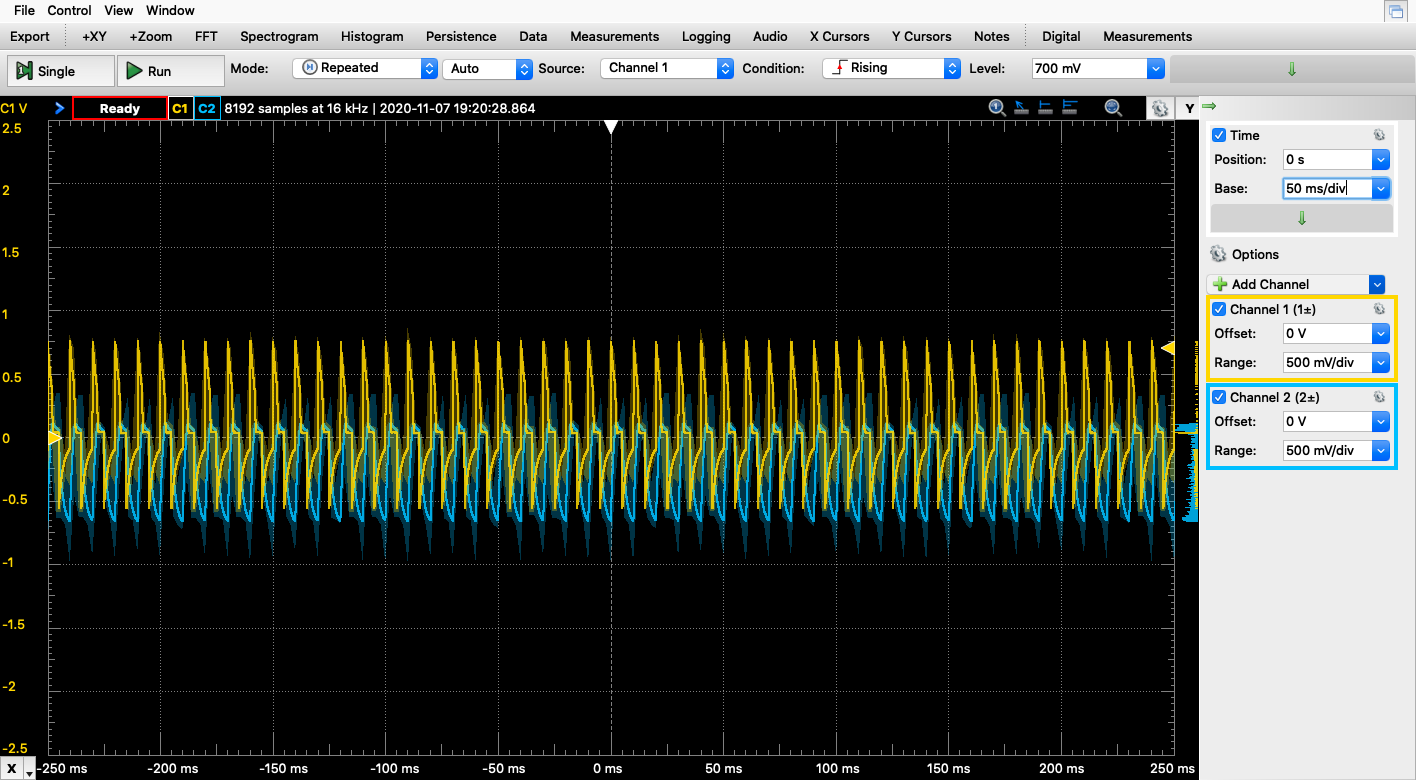
\includegraphics[scale=.15]{scope.png}
    \caption{$v_1$ (yellow) plotted on top of $v_o$ (blue)}
    \label{fig:scope}
\end{figure}
\begin{figure}[h]
    \centering
    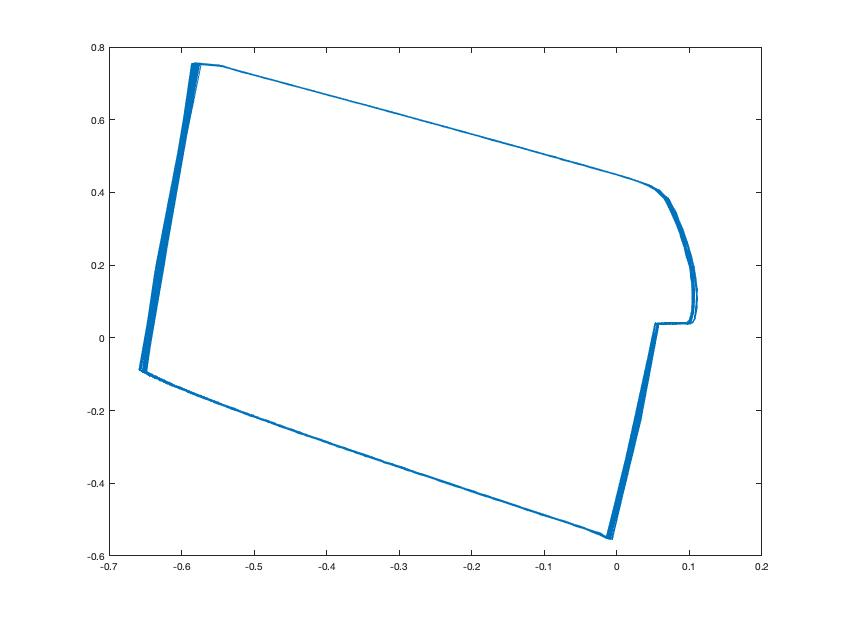
\includegraphics[scale=.3]{graph.jpg}
    \caption{$v_1$ plotted against $v_o$ using Matlab\textsuperscript{\tiny\textregistered}}
    \label{fig:scope}
\end{figure}
\section{Conclusion}
Utilizing Laplace transformations, an otherwise difficult differential equation was able to be solved using linear methods. The measurements of the circuit indicate an appropriate result, and though the author was not able to produce a true spiral, the two circular patterns at $90^{\circ}$ offsets are visible.

\end{document}
